\section{Fit model and signal extraction}
\label{sec:fit}

The parameter of interest in this search is the signal strength of the FCNC interactions, BR($t\to Hq$) and corresponding production mode cross section. The statistical analysis of the data employs a binned likelihood function constructed as the product of Poisson probability terms, in bins of the BDT output.

To take into account the systematic uncertianties associated with the MC estimation from different sources for both the signal and background samples, the fit model incorporates these systematics as extra Gaussian or Log-Normal constraint terms multiplied with the combined likelihood. The fitted central values and errors of the systematics parameters, or NPs, are expected to follow a normal distribution centered around 0 with unit width, when the Asimov data is used. The fit model construction is obtained with the \texttt{RooFit} and \texttt{RooStats} software, and the model configuration and persistence files (as input to \texttt{RooStats}) are produced by \texttt{TRExFitter} \cite{TRExFitter}, which is a software package interface with \texttt{HistFactory}. The \texttt{TRExFitter} includes additional features such as histogram smoothing, NP pruning and error symmetrization before the fits.
%A procedure called local symmetrization to the systematic variational histograms is implemented to semmetrize bins with one-sided variations which may cause problems in the fit.

The correlated bin-by-bin histogram variation corresponds to the up and down variation of each NP. The independent bin-by-bin fluctuations in the combined MC templates are also treated as NPs. They are incorporated in the model as extra Poisson constraint terms, and are expected to have a fitted value of 1 and a fitted error reflecting the relative statistical error in each particular bin. There is one parameter if interest (POI) freely floating in the fit without any constraints, namely, the signal strength $\mu$ (\texttt{SigXsecOverSM}) which is a multiplicative factor on a presumed branching ratio of BR($t\to Hq$)=$0.2\%$ in this analysis. The errors associated with the different systematics will be properly propogated to the fitted error of $\mu$ in a simultaneous fit of multiple regions via a profiled likelihood scan by the minimization program \texttt{MINUIT}. 

The one-sided NPs in the analysis, namely, \texttt{fakeSFXprongXPtbin}, \texttt{ttbar fragmentation}, \texttt{ttbar hard scattering}, \texttt{JET$\_$BJES$\_$Response}, \texttt{JET$\_$JER$\_$DataVsMC$\_$MC16}, \texttt{JET$\_$SingleParticle$\_$HighPt}, \texttt{JET$\_$TILECORR$\_$Uncertainty}, \texttt{MET$\_$SoftTrk$\_$ResoPara}, \texttt{MET$\_$SoftTrk$\_$ResoPerp} are symmetrized. This is done manually on the MC components of the background. By default, all the kinematic NPs (shape NPs due to, e.g., energy scales) are smoothed using the default smoothing parameters in \texttt{TRExFitter}. This helps removing the artificial NP constraints due to statistical fluctuations in the systematic variations, and makes the fit well behaved. The NPs pull distributions before the smoothing for each SR are given in App. \ref{app:channel_fit}.

Figure~\ref{fig:fcnc_rank_data} shows the ranking of the 25 top NPs along with their pull distributions, produced also with {\texttt TRExFitter}. The highest ranked NP is defined to have the largest impact on $\mu$. The impact is evalated by varying the NP under consideration by one $\sigma$ (either pre or post-fit error) up and down, and afterwards looking at the relative change in $\mu$ under the conditional fit where the NP under consideration is fixed to its varied new value.
Figure~\ref{fig:fcnc_pull_data} shows the pull distributions of all NPs in asimov fit. %The NPs which are constrained less than $80\%$ of their original error are smoothed with the default smoothing method in {\texttt TRExFitter}. The pre and post-smoothing distributions of the relevant NPs are given in App. \ref{app:smoothpruneNP}. Similar pull distributions before the NP smoothing are given in Fig. \ref{fig:fcnc_pull_nosmooth} of App. \ref{app:smoothpruneNP}.
Normalization and shape systematics whose impact is less than $1\%$ are removed from the fit. The list of removed NPs are given in App. \ref{app:smoothpruneNP}.

The NP ranking and constraints can be qualitatively understood from the variations of the BDT distributions due to the relevant NPs. Figures \ref{fig:NPvar_rank_data_a}-\ref{fig:NPvar_rank_data_d} show the systematic variations due to the top ranked NPs. %All of them cause large variations in the high-BDT signal region, hence are ranked high. The \texttt{THEORY\_RADIATION} is also constrained to $<80\%$ due to bins where the systematic variation is much bigger than the statistical one. However, after smoothing, this NP is not constrained any more. 

%The latter two cause large variation in the signal region, but small variation in the low BDT background region. Thus, they have large impact on the fitted signal strength but are not much constrained by the fit. The first one causes large variations in the background region, but it is an overall shift effect which can be adjusted by the fit through the floating normalization factors of the fake. Therefore, this NP is not constrained either. The \texttt{NOS\_TOPFRAC\_LH} only affects the $\tlhad$ channel, so the variation in $\thadhad$ is null. It causes up to $10\%$ bin-by-bin variations in both the signal and the background regions, which explains why it has a high ranking and is constrained at the same time.
%Figure \ref{fig:NPvar_other} shows the systematic variations due to a few constrained NPs, \texttt{JET\_JES\_PILEUP\_RHOTOPOLOGY}, \texttt{TAU\_TES\_INSITU} and \texttt{MET\_SOFTTRK\_RESOPERP}. They cause about $5-20\%$ bin-by-bin variations in the low BDT region, which can be constrained by the background region events. As a result, their impact on the signal is also reduced. Note that \texttt{MET\_SOFTTRK\_RESOPERP} is a one-sided NP, whose upward and downward variations are set to be the same.

Figure~\ref{fig:fcnc_correl_data} shows the correlation matrix for diffrent NPs. Except for self-correlations, and the correlations between the normalization factors (including POI) and the others, all the NPs have relatively small correlations with each other, which justifies the fit models for independent systematics. %Figure \ref{fig:sig_strength} shows the negative logrithm profile likelihood as a function of the signal strength (BR($t\to Hq$)=$1\%$ is assumed), with the $1\sigma$ confidence interval indicated. The best fit signal strength is $1.00_{-0.21}^{+0.25}$.


%\begin{figure}[htb]
%\centering
%\includegraphics[width=0.6\textwidth]{\FCNCFigures/r21/fit/4_mu.eps}
%\caption{ The best fit values of BR($t\to Hq$) in different channels from the S+B data fit. }
%\label{fig:4_mu}
%\end{figure}
%
%\begin{figure}[htb]
%\centering
%\includegraphics[width=0.6\textwidth]{\FCNCFigures/r21/fit/sig_inj.eps}
%\caption{ The best fit values of BR($t\to Hq$) from the S+B data fit, with different amount of FCNC signal injected into the real data. The blue %dashed line indicates the expected linear relation between the fitted and injected signal. }
%\label{fig:sig_inj}
%\end{figure}


\begin{figure}[htb]
\centering
\includegraphics[width=0.30\textwidth]{\FCNCFigures/r21/fit/tthml/reg1l1tau1b2j_os.eps}
\put(-100, 55){\textbf{(a1)}}
\put(-100, 45){\footnotesize{STH $\tlhad$}}
\includegraphics[width=0.30\textwidth]{\FCNCFigures/r21/fit/tthml/reg1l1tau1b2j_os_postFit.eps}
\put(-100, 55){\textbf{(a2)}}
\put(-100, 45){\footnotesize{STH $\tlhad$}}\\
\includegraphics[width=0.30\textwidth]{\FCNCFigures/r21/fit/tthml/reg1l1tau1b3j_os.eps}
\put(-100, 55){\textbf{(b1)}}
\put(-100, 45){\footnotesize{TTH $\tlhad$}}
\includegraphics[width=0.30\textwidth]{\FCNCFigures/r21/fit/tthml/reg1l1tau1b3j_os_postFit.eps}
\put(-100, 55){\textbf{(b2)}}
\put(-100, 45){\footnotesize{TTH $\tlhad$}}\\
\includegraphics[width=0.30\textwidth]{\FCNCFigures/r21/fit/tthml/reg1l2tau1bnj_os.eps}
\put(-100, 55){\textbf{(c1)}}
\put(-100, 45){\footnotesize{$l\thadhad$}}
\includegraphics[width=0.30\textwidth]{\FCNCFigures/r21/fit/tthml/reg1l2tau1bnj_os_postFit.eps}
\put(-100, 55){\textbf{(c2)}}
\put(-100, 45){\footnotesize{$l\thadhad$}}\\

\caption{ The asimov prefit (left) and postfit (right) BDT distributions in the STH $\tlhad$ (a1-2) and TTH $\tlhad$ (b1-2), $l\thadhad$ (c1-2)}
\label{fig:BDT_pre_post_sb_data}
\end{figure}

\begin{figure}[htb]
\centering
\includegraphics[width=0.30\textwidth]{\FCNCFigures/r21/fit/xtfw/reg2mtau1b3jos.eps}
\put(-100, 55){\textbf{(a1)}}
\put(-100, 45){\footnotesize{TTH $\thadhad$}}
\includegraphics[width=0.30\textwidth]{\FCNCFigures/r21/fit/xtfw/reg2mtau1b3jos_postFit.eps}
\put(-100, 55){\textbf{(a2)}}
\put(-100, 45){\footnotesize{TTH $\thadhad$}}\\
\includegraphics[width=0.30\textwidth]{\FCNCFigures/r21/fit/xtfw/reg2mtau1b2jos.eps}
\put(-100, 55){\textbf{(b1)}}
\put(-100, 45){\footnotesize{STH $\thadhad$}}
\includegraphics[width=0.30\textwidth]{\FCNCFigures/r21/fit/xtfw/reg2mtau1b2jos_postFit.eps}
\put(-100, 55){\textbf{(b2)}}
\put(-100, 45){\footnotesize{STH $\thadhad$}}

\caption{ The asimov prefit (left) and postfit (right) BDT distributions in the TTH $\thadhad$ (a1-2) and STH $\thadhad$ (b1-2)}
\label{fig:BDT_pre_post_sb_data}
\end{figure}

\begin{figure}[htb]
\centering
\includegraphics[width=0.45\textwidth]{\FCNCFigures/r21/fit/xtfw/NuisPar.eps}
\includegraphics[width=0.45\textwidth]{\FCNCFigures/r21/fit/tthml/NuisPar.eps}
\caption{ The asimov fit pull distributions of different NPs for $\thadhad$ channels (left) combined and lepton channels combined (right). }
\label{fig:fcnc_pull_sb_data}
\end{figure}

\begin{figure}[htb]
\centering
\includegraphics[width=0.45\textwidth]{\FCNCFigures/r21/fit/xtfw/RankingSysts.eps}
\includegraphics[width=0.45\textwidth]{\FCNCFigures/r21/fit/tthml/RankingSysts.eps}
%\put(-50, 150){\textbf{(a)}}
\caption{ The asimov fit ranking of the top 25 NPs for $\thadhad$ channels (left) combined and lepton channels combined (right). The scale of the relative impact on $\mu$ (the pull) of the NPs is shown on the top (bottom) axis.}
\label{fig:fcnc_rank_data}
\end{figure}

\begin{figure}[htb]
\centering
\includegraphics[width=0.45\textwidth]{\FCNCFigures/r21/fit/xtfw/CorrMatrix.eps}
\includegraphics[width=0.45\textwidth]{\FCNCFigures/r21/fit/tthml/CorrMatrix.eps}
%\put(-50, 150){\textbf{(a)}}
\caption{ The asimov fit correlation matrix ($\%$) of different NPs, with a threshold of $20\%$ for $\thadhad$ channels (left) combined and lepton channels combined (right). }
\label{fig:fcnc_correl_data}
\end{figure}

%\begin{figure}[htb]
%\centering
%\includegraphics[width=0.32\textwidth]{\FCNCFigures/r21/fit/var_rank1_hh_4j_data.eps}
%\put(-45, 65){\footnotesize{$hh$ 4-jet}}
%\includegraphics[width=0.32\textwidth]{\FCNCFigures/r21/fit/var_rank2_hh_4j_data.eps}
%\put(-45, 65){\footnotesize{$hh$ 4-jet}}
%\includegraphics[width=0.32\textwidth]{\FCNCFigures/r21/fit/var_rank3_hh_4j_data.eps}
%\put(-45, 65){\footnotesize{$hh$ 4-jet}}\\
%\includegraphics[width=0.32\textwidth]{\FCNCFigures/r21/fit/var_rank1_hh_3j_data.eps}
%\put(-45, 65){\footnotesize{$hh$ 3-jet}}
%\includegraphics[width=0.32\textwidth]{\FCNCFigures/r21/fit/var_rank2_hh_3j_data.eps}
%\put(-45, 65){\footnotesize{$hh$ 3-jet}}
%\includegraphics[width=0.32\textwidth]{\FCNCFigures/r21/fit/var_rank3_hh_3j_data.eps}
%\put(-45, 65){\footnotesize{$hh$ 3-jet}}\\
%\includegraphics[width=0.32\textwidth]{\FCNCFigures/dummy_600_450.eps}
%\includegraphics[width=0.32\textwidth]{\FCNCFigures/r21/fit/var_rank2_lh_4j_data.eps}
%\put(-45, 65){\footnotesize{$lh$ 4-jet}}
%\includegraphics[width=0.32\textwidth]{\FCNCFigures/r21/fit/var_rank3_lh_4j_data.eps}
%\put(-45, 65){\footnotesize{$lh$ 4-jet}}\\
%\includegraphics[width=0.32\textwidth]{\FCNCFigures/dummy_600_450.eps}
%\includegraphics[width=0.32\textwidth]{\FCNCFigures/r21/fit/var_rank2_lh_3j_data.eps}
%\put(-45, 65){\footnotesize{$lh$ 3-jet}}
%\includegraphics[width=0.32\textwidth]{\FCNCFigures/r21/fit/var_rank3_lh_3j_data.eps}
%\put(-45, 65){\footnotesize{$lh$ 3-jet}}\\
%\caption{ The prefit variations of BDT distributions (B-only) due to the three top ranked NPs with the unblinded data, \texttt{nos\_topFrac\_hh} (%left), \texttt{jet\_jer} (middle) and \texttt{theory\_ME} (right). Form top to bottom rows: $\thadhad$ 4-jet, $\thadhad$ 3-jet, $\tlhad$ 4-jet, $\%tlhad$ 3-jet. }
%\label{fig:NPvar_rank_data_a}
%\end{figure}
%
%\begin{figure}[htb]
%\centering
%\includegraphics[width=0.32\textwidth]{\FCNCFigures/r21/fit/var_rank4_hh_4j_data.eps}
%\put(-45, 65){\footnotesize{$hh$ 4-jet}}
%\includegraphics[width=0.32\textwidth]{\FCNCFigures/r21/fit/var_rank5_hh_4j_data.eps}
%\put(-45, 65){\footnotesize{$hh$ 4-jet}}
%\includegraphics[width=0.32\textwidth]{\FCNCFigures/r21/fit/var_rank6_hh_4j_data.eps}
%\put(-45, 65){\footnotesize{$hh$ 4-jet}}\\
%\includegraphics[width=0.32\textwidth]{\FCNCFigures/r21/fit/var_rank4_hh_3j_data.eps}
%\put(-45, 65){\footnotesize{$hh$ 3-jet}}
%\includegraphics[width=0.32\textwidth]{\FCNCFigures/r21/fit/var_rank5_hh_3j_data.eps}
%\put(-45, 65){\footnotesize{$hh$ 3-jet}}
%\includegraphics[width=0.32\textwidth]{\FCNCFigures/r21/fit/var_rank6_hh_3j_data.eps}
%\put(-45, 65){\footnotesize{$hh$ 3-jet}}\\
%\includegraphics[width=0.32\textwidth]{\FCNCFigures/r21/fit/var_rank4_lh_4j_data.eps}
%\put(-45, 65){\footnotesize{$lh$ 4-jet}}
%\includegraphics[width=0.32\textwidth]{\FCNCFigures/r21/fit/var_rank5_lh_4j_data.eps}
%\put(-45, 65){\footnotesize{$lh$ 4-jet}}
%\includegraphics[width=0.32\textwidth]{\FCNCFigures/r21/fit/var_rank6_lh_4j_data.eps}
%\put(-45, 65){\footnotesize{$lh$ 4-jet}}\\
%\includegraphics[width=0.32\textwidth]{\FCNCFigures/r21/fit/var_rank4_lh_3j_data.eps}
%\put(-45, 65){\footnotesize{$lh$ 3-jet}}
%\includegraphics[width=0.32\textwidth]{\FCNCFigures/r21/fit/var_rank5_lh_3j_data.eps}
%\put(-45, 65){\footnotesize{$lh$ 3-jet}}
%\includegraphics[width=0.32\textwidth]{\FCNCFigures/r21/fit/var_rank6_lh_3j_data.eps}
%\put(-45, 65){\footnotesize{$lh$ 3-jet}}\\
%\caption{ The prefit variations of BDT distributions (B-only) due to the 4th-6th ranked NPs with the unblinded data, \texttt{btag\_light\_10} (left)%, \texttt{jet\_jes\_etaintercalibration\_modelling} (middle) and \texttt{tau\_eff\_jetid\_total} (right). Form top to bottom rows: $\thadhad$ 4-jet, %$\thadhad$ 3-jet, $\tlhad$ 4-jet, $\tlhad$ 3-jet. }
%\label{fig:NPvar_rank_data_b}
%\end{figure}
%
%\begin{figure}[htb]
%\centering
%\includegraphics[width=0.32\textwidth]{\FCNCFigures/r21/fit/var_rank7_hh_4j_data.eps}
%\put(-45, 65){\footnotesize{$hh$ 4-jet}}
%\includegraphics[width=0.32\textwidth]{\FCNCFigures/r21/fit/var_rank8_hh_4j_data.eps}
%\put(-45, 65){\footnotesize{$hh$ 4-jet}}
%\includegraphics[width=0.32\textwidth]{\FCNCFigures/r21/fit/var_rank9_hh_4j_data.eps}
%\put(-45, 65){\footnotesize{$hh$ 4-jet}}\\
%\includegraphics[width=0.32\textwidth]{\FCNCFigures/r21/fit/var_rank7_hh_3j_data.eps}
%\put(-45, 65){\footnotesize{$hh$ 3-jet}}
%\includegraphics[width=0.32\textwidth]{\FCNCFigures/r21/fit/var_rank8_hh_3j_data.eps}
%\put(-45, 65){\footnotesize{$hh$ 3-jet}}
%\includegraphics[width=0.32\textwidth]{\FCNCFigures/r21/fit/var_rank9_hh_3j_data.eps}
%\put(-45, 65){\footnotesize{$hh$ 3-jet}}\\
%\includegraphics[width=0.32\textwidth]{\FCNCFigures/r21/fit/var_rank7_lh_4j_data.eps}
%\put(-45, 65){\footnotesize{$lh$ 4-jet}}
%\includegraphics[width=0.32\textwidth]{\FCNCFigures/r21/fit/var_rank8_lh_4j_data.eps}
%\put(-45, 65){\footnotesize{$lh$ 4-jet}}
%\includegraphics[width=0.32\textwidth]{\FCNCFigures/r21/fit/var_rank9_lh_4j_data.eps}
%\put(-45, 65){\footnotesize{$lh$ 4-jet}}\\
%\includegraphics[width=0.32\textwidth]{\FCNCFigures/r21/fit/var_rank7_lh_3j_data.eps}
%\put(-45, 65){\footnotesize{$lh$ 3-jet}}
%\includegraphics[width=0.32\textwidth]{\FCNCFigures/r21/fit/var_rank8_lh_3j_data.eps}
%\put(-45, 65){\footnotesize{$lh$ 3-jet}}
%\includegraphics[width=0.32\textwidth]{\FCNCFigures/r21/fit/var_rank9_lh_3j_data.eps}
%\put(-45, 65){\footnotesize{$lh$ 3-jet}}\\
%\caption{ The prefit variations of BDT distributions (B-only) due to the 7th-9th ranked NPs with the unblinded data, \texttt{jet\_jes\_flavor\_%composition} (left), \texttt{btag\_light\_9} (middle) and \texttt{jet\_jes\_pileup\_rhotopology} (right). Form top to bottom rows: $\thadhad$ 4-jet, %$\thadhad$ 3-jet, $\tlhad$ 4-jet, $\tlhad$ 3-jet. }
%\label{fig:NPvar_rank_data_c}
%\end{figure}
%
%\begin{figure}[htb]
%\centering
%\includegraphics[width=0.32\textwidth]{\FCNCFigures/r21/fit/var_extra1_hh_4j_data.eps}
%\put(-45, 65){\footnotesize{$hh$ 4-jet}}
%\includegraphics[width=0.32\textwidth]{\FCNCFigures/r21/fit/var_extra2_hh_4j_data.eps}
%\put(-45, 65){\footnotesize{$hh$ 4-jet}}
%\includegraphics[width=0.32\textwidth]{\FCNCFigures/r21/fit/var_extra3_hh_4j_data.eps}
%\put(-45, 65){\footnotesize{$hh$ 4-jet}}\\
%\includegraphics[width=0.32\textwidth]{\FCNCFigures/r21/fit/var_extra1_hh_3j_data.eps}
%\put(-45, 65){\footnotesize{$hh$ 3-jet}}
%\includegraphics[width=0.32\textwidth]{\FCNCFigures/r21/fit/var_extra2_hh_3j_data.eps}
%\put(-45, 65){\footnotesize{$hh$ 3-jet}}
%\includegraphics[width=0.32\textwidth]{\FCNCFigures/r21/fit/var_extra3_hh_3j_data.eps}
%\put(-45, 65){\footnotesize{$hh$ 3-jet}}\\
%\includegraphics[width=0.32\textwidth]{\FCNCFigures/r21/fit/var_extra1_lh_4j_data.eps}
%\put(-45, 65){\footnotesize{$lh$ 4-jet}}
%\includegraphics[width=0.32\textwidth]{\FCNCFigures/r21/fit/var_extra2_lh_4j_data.eps}
%\put(-45, 65){\footnotesize{$lh$ 4-jet}}
%\includegraphics[width=0.32\textwidth]{\FCNCFigures/r21/fit/var_extra3_lh_4j_data.eps}
%\put(-45, 65){\footnotesize{$lh$ 4-jet}}\\
%\includegraphics[width=0.32\textwidth]{\FCNCFigures/r21/fit/var_extra1_lh_3j_data.eps}
%\put(-45, 65){\footnotesize{$lh$ 3-jet}}
%\includegraphics[width=0.32\textwidth]{\FCNCFigures/r21/fit/var_extra2_lh_3j_data.eps}
%\put(-45, 65){\footnotesize{$lh$ 3-jet}}
%\includegraphics[width=0.32\textwidth]{\FCNCFigures/r21/fit/var_extra3_lh_3j_data.eps}
%\put(-45, 65){\footnotesize{$lh$ 3-jet}}\\
%\caption{ The prefit variations of BDT distributions (B-only) due to a few other NPs with the unblinded data, \texttt{btag\_light\_12} (left), \%texttt{jet\_jes\_etaintercalibration\_totalstat} (middle) and \texttt{jet\_jes\_flavor\_response} (right). Form top to bottom rows: $\thadhad$ 4-%jet, $\thadhad$ 3-jet, $\tlhad$ 4-jet, $\tlhad$ 3-jet. }
%\label{fig:NPvar_rank_data_d}
%\end{figure}
